%% LyX 2.2.2 created this file.  For more info, see http://www.lyx.org/.
%% Do not edit unless you really know what you are doing.
\documentclass[english]{beamer}
\usepackage[T1]{fontenc}
\usepackage[latin9]{luainputenc}
\setcounter{secnumdepth}{3}
\setcounter{tocdepth}{3}
\usepackage{graphicx}

\makeatletter

%%%%%%%%%%%%%%%%%%%%%%%%%%%%%% LyX specific LaTeX commands.
%% Because html converters don't know tabularnewline
\providecommand{\tabularnewline}{\\}

%%%%%%%%%%%%%%%%%%%%%%%%%%%%%% Textclass specific LaTeX commands.
 % this default might be overridden by plain title style
 \newcommand\makebeamertitle{\frame{\maketitle}}%
 % (ERT) argument for the TOC
 \AtBeginDocument{%
   \let\origtableofcontents=\tableofcontents
   \def\tableofcontents{\@ifnextchar[{\origtableofcontents}{\gobbletableofcontents}}
   \def\gobbletableofcontents#1{\origtableofcontents}
 }

%%%%%%%%%%%%%%%%%%%%%%%%%%%%%% User specified LaTeX commands.

\usetheme{CambridgeUS}
\usepackage[position=top]{subfig}

\definecolor{UBCblue}{rgb}{0.04706, 0.13725, 0.26667} % UBC Blue (primary)
\definecolor{UBCgrey}{rgb}{0.3686, 0.5255, 0.6235} % UBC Grey (secondary)
\setbeamercolor{palette primary}{bg=UBCblue,fg=white}
\setbeamercolor{palette secondary}{bg=UBCblue,fg=white}
\setbeamercolor{palette tertiary}{bg=UBCblue,fg=white}
\setbeamercolor{palette quaternary}{bg=UBCblue,fg=white}
\setbeamercolor{structure}{fg=UBCblue} % itemize, enumerate, etc
\setbeamercolor{section in toc}{fg=UBCblue} % TOC sections
% Override palette coloring with secondary
\setbeamercolor{subsection in head/foot}{bg=UBCgrey,fg=white}

\useinnertheme{rectangles}
\useoutertheme{infolines}

\setbeamercolor{title}{fg=UBCblue,bg=UBCblue!20}
\setbeamercolor{frametitle}{fg=UBCblue,bg=UBCblue!20}
\setbeamercolor{section in head/foot}{bg=UBCblue}
\setbeamercolor{author in head/foot}{bg=UBCblue}
\setbeamercolor{date in head/foot}{fg=UBCblue}

\@ifundefined{showcaptionsetup}{}{%
 \PassOptionsToPackage{caption=false}{subfig}}
\usepackage{subfig}
\makeatother

\usepackage{babel}
\begin{document}

\title{CNN Quantization}

\subtitle{Performance evaluation}

\author{Emanuele Ghelfi \and Emiliano Gagliardi}

\titlegraphic{Politecnico di Milano}
\makebeamertitle
\begin{frame}

\frametitle<presentation>{Contents}

\tableofcontents{}
\end{frame}

\section{Purposes}
\begin{frame}{Project purpose}

Using a machine learning framework with support for convolutional
neural networks
\begin{itemize}
\item Define different kind of networks
\item Train
\item Quantize
\item Evaluate the original and the quantized models
\item Make a comparison in term of size of the model, cache misses, and
inference time
\end{itemize}
\end{frame}

\section{Quantization}
\begin{frame}{What is quantization?}

Developing this project we saw two different approaches:
\begin{itemize}
\item Tensorflow
\item Caffe Ristretto
\end{itemize}
\end{frame}
%
\begin{frame}{Tensorflow quantization}

\noindent %
\begin{minipage}[c][1\totalheight][t]{0.55\columnwidth}%
Unsupervised approach
\begin{itemize}
\item Get a trained network
\item Obtain for each layer the min and the max of the weights value
\item Represent the weights distributed linearly between the minimum and
maximum with 8 bits precision
\item The operations have to be reimplemented for the 8-bit format
\end{itemize}
%
\end{minipage}%
\begin{minipage}[c][1\totalheight][t]{0.45\columnwidth}%
\begin{center}
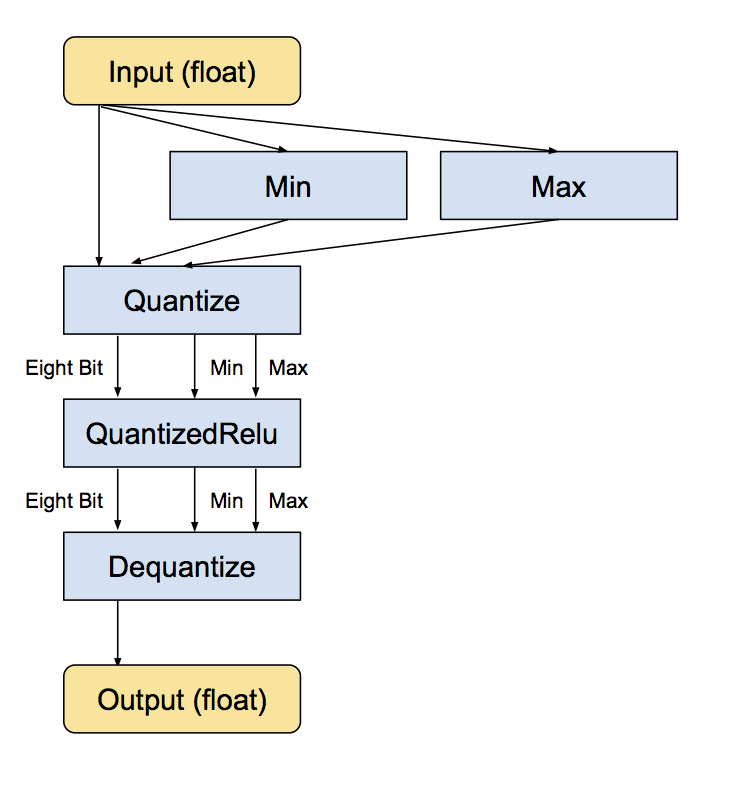
\includegraphics[width=0.4\paperwidth]{images/tensorflow-quantization}
\par\end{center}%
\end{minipage}\\
The resulting data structure is composed by an array containing the
quantized value, and the two float min and max
\end{frame}
%
\begin{frame}{Caffe Ristretto quantization}

Supervised approach
\begin{itemize}
\item Get a trained network
\item Three different methods:
\begin{itemize}
\item Dynamic fixed point: a modified fixed-point format
\item Minifloat: bit-width reduced floating point numbers
\item Power of two: layers with power-of-two parameters don\textquoteright t
need any multipliers, when implemented in hardware
\end{itemize}
\item Evaluate the performance of the network during quantization in order
to keep the accuracy higher than a given threshold
\item Support for training of quantized networks (fine-tuning)
\end{itemize}
\end{frame}
%
\begin{frame}{Caff� Ristretto quantization}

\begin{figure}

\centering{}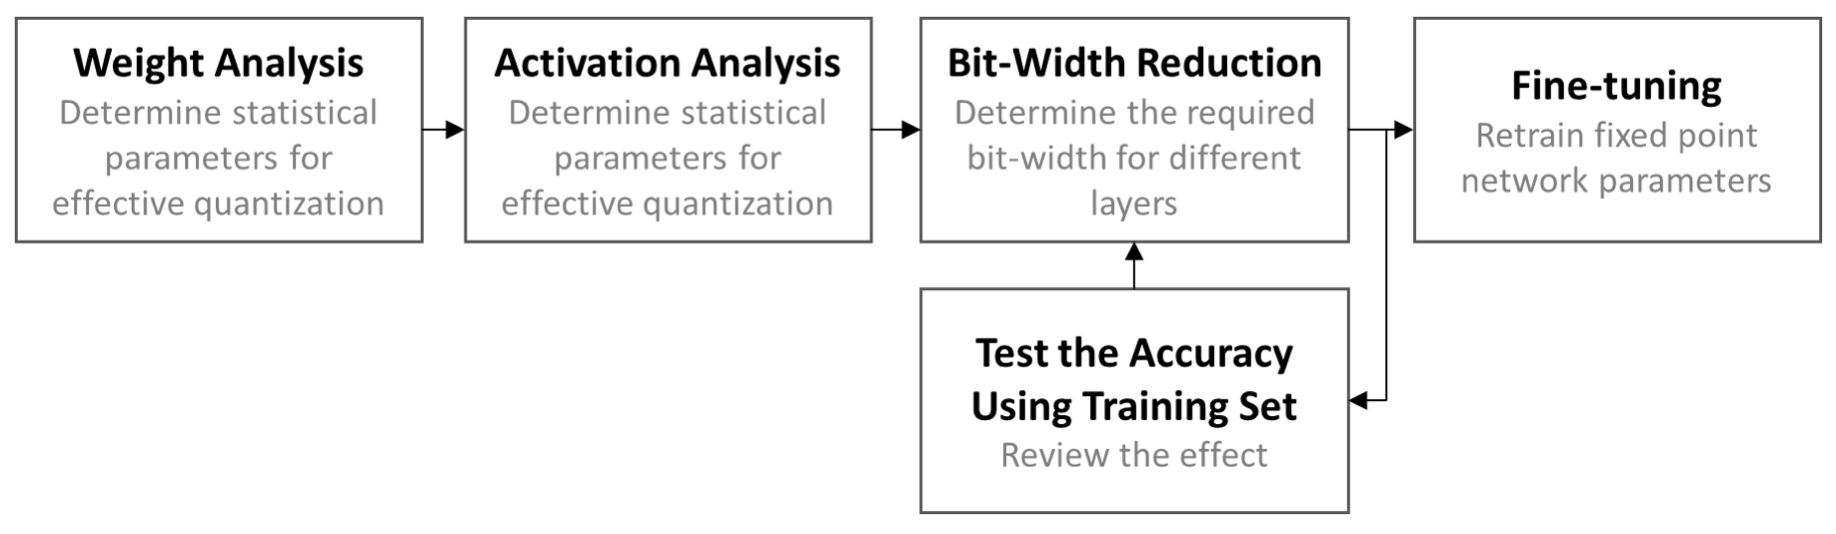
\includegraphics[width=0.9\paperwidth]{images/ristretto-quantization}
\end{figure}
\end{frame}
%
\begin{frame}{Why quantize?}

Accuracy/inference speed trade-off
\begin{itemize}
\item Deep networks tend to cope very well with high levels of noise in
their inputs.
\item It seems that there is no need of floating point precision
\item Training still needs floating point precision to work, it is an iteration
of little incremental adjustments of the weights
\end{itemize}
So deep networks are trained with floating point precision, then a
quantization algorithm can be applied to obtain smaller models and
speed up the inference phase
\end{frame}
%

\section{Our work}
\begin{frame}{Caffe ristretto}

The results obtained with Ristretto on a simple network for the Mnist
dataset are not so satisfying...
\begin{figure}
\noindent \begin{centering}
\begin{tabular}{|c|c|c|c|c|c|}
\hline 
\textcolor{black}{\tiny{}network} & \textcolor{black}{\tiny{}accuracy} & \textcolor{black}{\tiny{}model size (MB)} & \textcolor{black}{\tiny{}Time (ms)} & \textcolor{black}{\tiny{}LL\_d misses ($10^{6}$)} & \textcolor{black}{\tiny{}L1\_d misses ($10^{6}$) }\tabularnewline
\hline 
\textcolor{black}{\tiny{}Orginal} & \textcolor{black}{\tiny{}0.9903} & \textcolor{red}{\tiny{}1.7} & \textcolor{black}{\tiny{}29.2} & \textcolor{black}{\tiny{}32.098} & \textcolor{black}{\tiny{}277.189}\tabularnewline
\hline 
\textcolor{black}{\tiny{}Dynamic f. p.} & \textcolor{black}{\tiny{}0.9829} & \textcolor{red}{\tiny{}1.7} & \textcolor{black}{\tiny{}126.41} & \textcolor{black}{\tiny{}42.077} & \textcolor{black}{\tiny{}303.209}\tabularnewline
\hline 
\textcolor{black}{\tiny{}Minifloat} & \textcolor{black}{\tiny{}0.9916} & \textcolor{red}{\tiny{}1.7} & \textcolor{black}{\tiny{}29.5} & \textcolor{black}{\tiny{}37.149} & \textcolor{black}{\tiny{}282.396}\tabularnewline
\hline 
\textcolor{black}{\tiny{}Power of two} & \textcolor{black}{\tiny{}0.9899} & \textcolor{red}{\tiny{}1.7} & \textcolor{black}{\tiny{}61.1} & \textcolor{black}{\tiny{}35.774} & \textcolor{black}{\tiny{}280.819}\tabularnewline
\hline 
\end{tabular}
\par\end{centering}
\textcolor{black}{\tiny{}Linux running on macbook pro, cachegrind
tool for cache statistics. Intel i5 2.9 GHz, L3 cache 3MB, 16 GB ram.}{\tiny \par}
\end{figure}

\begin{itemize}
\item The quantized values are stored in float size after the quantization
\item The quantized layers implementation works with float variables:
\begin{itemize}
\item perform the computation with low precision values stored in float
variables
\item quantize the results, still stored in float variables
\end{itemize}
\end{itemize}
\end{frame}
%
\begin{frame}{Tensorflow}

The quantization is better supported
\begin{itemize}
\item The quantized model is stored with low precision weights
\item Some low precision operations are already implemented
\end{itemize}
We tried different topologies of networks, to see how quantization
affect different architectures
\end{frame}
%
\begin{frame}{How we used the tensorflow quantization tool}
\begin{itemize}
\item We used python (with a bit OO, since we needed a way to use it with
different networks)
\item An abstract class defines the pattern of the network that the main
script can handle
\item The core methods of the pattern are
\begin{itemize}
\item prepare: build the computational graph of the network and the training
step, load the data
\item train: iterate the train step
\end{itemize}
\item The main script takes in input an instance and:
\begin{itemize}
\item calls prepare and train
\item quantizes the obtained network
\item evaluates the accuracy 
\item evaluates cache performance using linux-perf
\item plots the data
\end{itemize}
\end{itemize}
\end{frame}
%
\begin{frame}{Topologies}
\noindent \begin{center}
\begin{figure}[t]
\noindent \centering{}\subfloat[big]{\noindent \begin{centering}
\par\end{centering}
\noindent \centering{}\includegraphics[width=0.15\paperwidth,height=0.7\textheight]{\string"images/network topologies/big2conv_3fc\string".png}}\hfill{}\subfloat[more conv]{\noindent \begin{centering}
\par\end{centering}
\noindent \begin{centering}
\includegraphics[width=0.15\paperwidth,height=0.7\textheight]{\string"images/network topologies/bigconv_small_fc\string".png}
\par\end{centering}
}\hfill{}\subfloat[more FC]{\noindent \begin{centering}
\par\end{centering}
\noindent \begin{centering}
\includegraphics[width=0.15\paperwidth,height=0.7\textheight]{\string"images/network topologies/small_conv_bigfc\string".png}
\par\end{centering}
}\hfill{}\subfloat[tf example]{\noindent \begin{centering}
\par\end{centering}
\noindent \centering{}\includegraphics[width=0.15\paperwidth,height=0.7\textheight]{\string"images/network topologies/2conv2fc\string".png}}\hfill{}\subfloat[only FC]{\noindent \begin{centering}
\par\end{centering}
\noindent \centering{}\includegraphics[width=0.15\paperwidth]{\string"images/network topologies/3fc\string".png}}
\end{figure}
\par\end{center}

\end{frame}
%
\begin{frame}{Some data - accuracy}

\noindent 
\begin{figure}
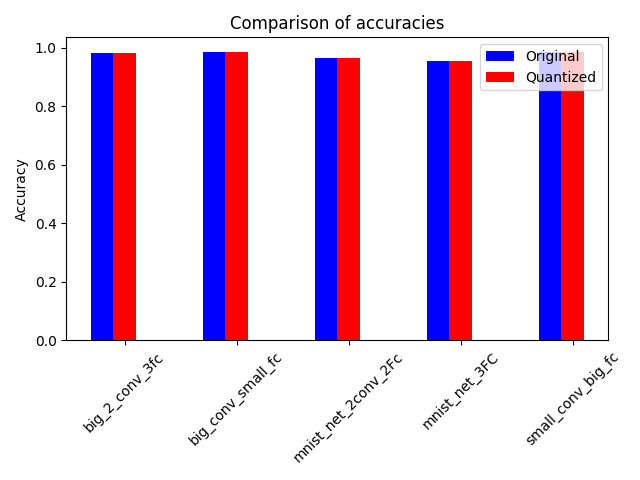
\includegraphics[width=1\paperheight]{images/tf-results/acc}
\end{figure}

\end{frame}
%
\begin{frame}{Some data - models size}

\begin{figure}
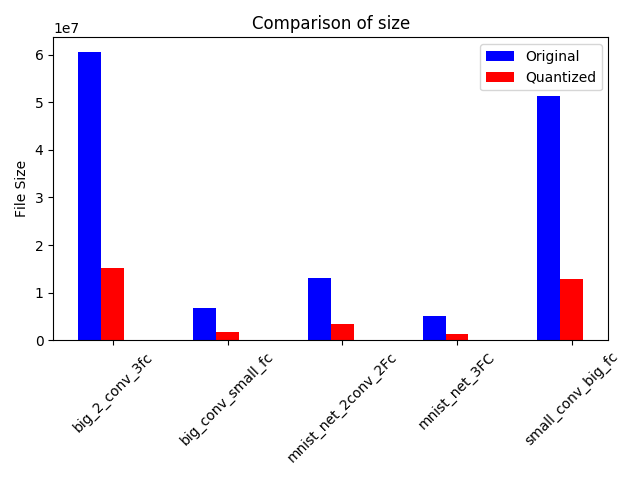
\includegraphics[width=0.75\paperwidth]{images/tf-results/size}
\end{figure}

\end{frame}
%
\begin{frame}{Some data - data cache misses}

\begin{figure}
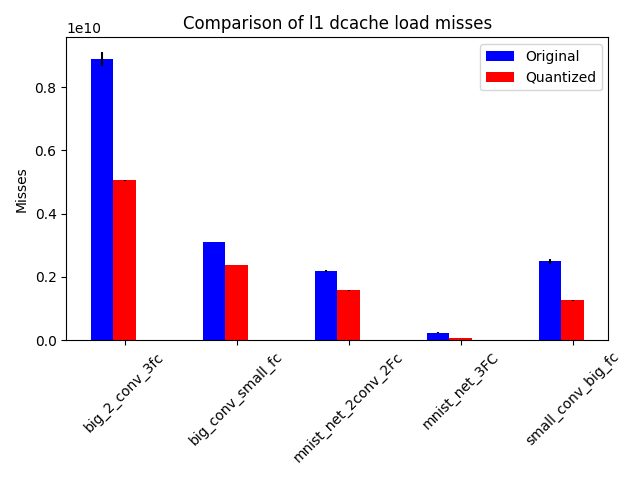
\includegraphics[width=0.75\paperwidth]{images/tf-results/misses}
\end{figure}

\end{frame}
%
\begin{frame}{Some data - inference time}

\begin{figure}
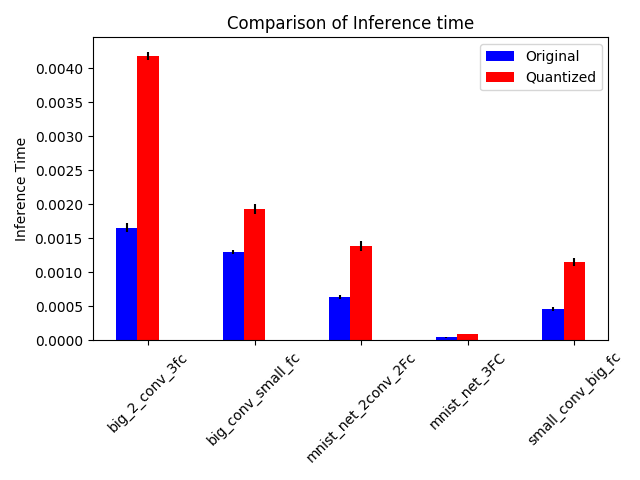
\includegraphics[width=0.75\paperwidth]{images/tf-results/test_time}
\end{figure}

\end{frame}
%
\begin{frame}{Why is the inference time worst?}
\begin{itemize}
\item We see an improvement in performance only for the size of the model,
and so for the data cache misses
\item Inference time and last level cache misses are worst in quantized
networks
\end{itemize}
From the tensorflow github page:

Only a subset of ops are supported, and on many platforms the quantized
code may actually be slower than the float equivalents, but this is
a way of increasing performance substantially when all the circumstances
are right.
\end{frame}
%
\begin{frame}{Original net - tensorflow benchmark tool}

\begin{figure}[t]
\includegraphics[width=0.85\paperwidth]{\string"images/tf benchmark tool/original perf\string".png}
\end{figure}

\end{frame}
%
\begin{frame}{Quantized net - tensorflow benchmark tool}

\begin{figure}[t]
\includegraphics[width=0.85\paperwidth]{\string"images/tf benchmark tool/quantized perf\string".png}
\end{figure}

\end{frame}
%
\begin{frame}{References}
\begin{itemize}
\item Tensorflow: https://www.tensorflow.org
\item Ristretto: http://lepsucd.com/?page\_id=621
\item Github repository of the project: \\
https://github.com/EmilianoGagliardiEmanueleGhelfi/CNN-compression-performance
\end{itemize}
\end{frame}

\end{document}
